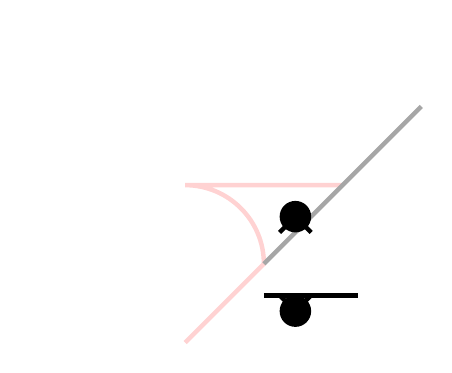
\begin{tikzpicture}[scale=2]

% Define the colors
\colorlet{unicornwhite}{white}
\colorlet{unicornblue}{gray!70}
\colorlet{unicornpink}{pink!70}

% Draw the body
\fill[unicornwhite] (0,0) -- (1,1) arc (0:180:1) -- cycle;

% Draw the mane
\draw[ultra thick, unicornpink] (0,0) -- (0.5,0.5) arc (0:90:0.5) -- (1,1);

% Draw the horn
\draw[ultra thick, unicornblue] (0.5,0.5) -- (1.5,1.5);

% Draw the eyes
\fill[black] (0.7,0.8) circle (0.1);
\fill[black] (0.7,0.2) circle (0.1);

% Draw the eyelashes
\draw[ultra thick, black] (0.7,0.8) -- (0.8,0.7);
\draw[ultra thick, black] (0.7,0.8) -- (0.6,0.7);
\draw[ultra thick, black] (0.7,0.2) -- (0.8,0.3);
\draw[ultra thick, black] (0.7,0.2) -- (0.6,0.3);

% Draw the mouth
\draw[ultra thick, black] (0.5,0.3) -- (1.1,0.3);

\end{tikzpicture}